\section{Research Goals}

\begin{figure}
	\centering
	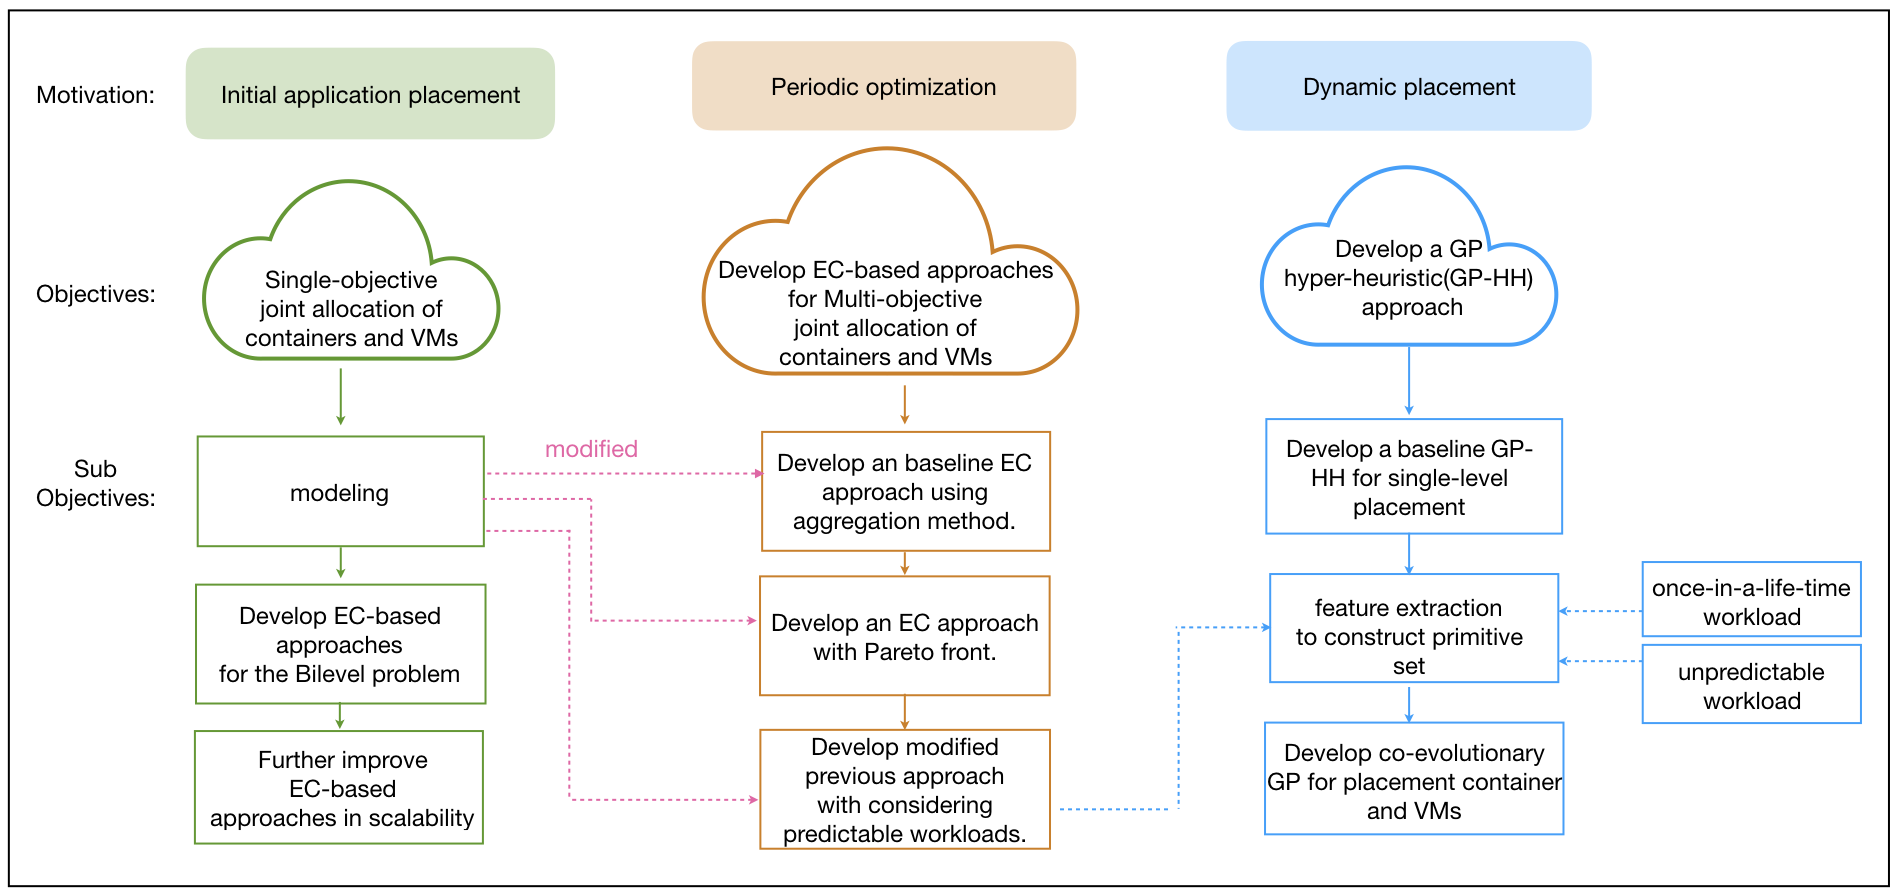
\includegraphics[width=\textwidth]{pics/thesisPlan.png}
	\caption{Relationship between objectives}
	\label{fig:objectives}
\end{figure}
\bx{The overall goal of this research is to optimize energy consumption of a container-based Cloud data center using EC-based approaches for three placement decision scenarios:} application initial placement, periodic optimization, and dynamic placement. The specific research objectives of this work can be itemized as follows.
% In this thesis, we aims at providing a series of approaches to continuously optimize the a joint allocation of VMs and containers that considers three consolidation scenarios: Initialization, global consolidation, Dynamic consolidation. In addition, the static allocation normally involves with large amount of variables which is particular difficult to optimize. We are also going to propose a method to solve this problem.  These approaches combine element of AI planning, to ensure the objectives and constraint fulfillment, and of Evolutionary Computation, to evolve a population of near-optimal solutions. The research aims at determining a flexible way in creation of solutions to solve server consolidation problems. As discussed in the previous section, the research goal can be achieved in the following objectives and sub-objectives.

\subsection{Objective One: Develop EC-based approaches for the single objective joint placement of containers and VMs for application initial placement}
\label{sec:obj1}

\bx{The goal is to reduce the energy consumption in application initial placement considering container-based cloud data center.} To achieve this goal, the first step is to propose a new bilevel model for the joint placement of containers and VMs problem which considers the problem as a bilevel optimization problem. We will explore evolutionary computation based approaches to solve the bievel problem (For the sake of simplicity, we will use ``the bilevel model/problem'' to replace ``the joint placement of containers and VMs model/problem'' in the following content.). The research goal leads to three objectives as follows. 
% \textcolor{Maroon}{Currently, most research on container consolidation do not consider the two-level of allocation problem.} Unlike previous VM-based service consolidation, 
% most research focus on VM-based server consolidation technique. They often modeled the VM allocation problem as a vector bin-packing problem \cite{Zhang:2016cx}. 
% Container adds an extra layer of abstraction on top of VM. The placement problem has become a two-step procedure, in the first step, containers are packed into VMs and then VMs are consolidated into physical machines. These two steps are inter-related to each other. Previous research \cite{Piraghaj:2015uf} solve this problem in separated steps where the first step allocates containers to VMs and the second step allocates VMs to PMs with simple bin-packing heuristics. According to Mann's \cite{Mann:2016hx} observation, these two allocations should be conducted simultaneously to reach a near-optima solution, which essentially minimizes the energy consumption.

\begin{enumerate}
	\item Develop a new bilevel model to capture the relationship between containers allocation and energy consumption in container-based cloud data center.
	% \textcolor{Maroon}{This problem can be considered as a bilevel problem \cite{} the lower-level optimization: allocate containers to VMs and the upper-level: allocate VMs to PMs.} 
	% \textcolor{Maroon}{Since the existing models for container-based consolidation are based on VM-based model which incurs two problems.}
	% First problem is that they did not consider the interaction between two levels of allocation.
	% Second problem is that they did not consider balancing the residual resources (e.g between CPU and memory). 
	\bx{The goal of the first sub objective is to propose a bilevel model for the joint placement of container and VM.} 

	\bx{The major challenge is that no previous research considers the joint placement container and VM as a bilevel problem while the relationship between container, VM and energy consumption is unclear.} Specifically, three issues remain unsolved. 
	The first issue is that it is still unclear that which energy function is the best to capture the relationship between container and VM so that the overall energy is low. Specifically, the objective for the upper level - placing container to VM, is still unclear. This is because the minimum number of VM does not necessary lead to the minimum number PMs; the types of VM also play an important role.
	The second issue is that previous VM-based research do not consider the overhead of VM. However, the overhead of VMs is a major source of resource wastage (addressed in Section \ref{sec:comparison_container_vm}). Therefore, how to represent the impact of VMs remains unsolved.
	The third issue is related to a VM-based research,  Mishra \cite{Mishra:2011bz} discovers that when multiple resources are considered in the model, the balance between resources has a heavy impact on the optimization results. Therefore, in the bilevel model, the balance of resources should also be considered.

	In order to establish a bilevel model, variables, constraints and objective functions need to be clarified before applying any optimization algorithm. Each level of the problem will be formulated to a multi-dimensional vector bin packing problem. 
	We will start from the simplest case - single dimension of resource - to more general multi-dimensional resources model by reviewing a number of VM-based approaches. Specifically, we focus on their variables, constraints and objective function. Objective function is mainly related to energy consumption. Hence, energy model is another major issue to study. In addition, in the multi-dimensional resource model, we will address the balance of CPU and memory problem by investigating several resource wastage models \cite{Ferdaus:2014ep, Xu:2010vh, Gao:2013gg}. In this objective, we consider the static workload of applications, this is because the initial resource demand is often provided by the Cloud users.

	\item Propose a new EC based bilevel optimization approach to solve the application initial placement.\\
	\bx{Based on the proposed bilevel model, the goal of this sub-objective is to develop an approach for the bilevel optimization problem using nested Evolutionary algorithms \cite{Sinha:2017et}.}

	\bx{Three challenges need to be solved. First one is to understand the interaction between bilevel's placement.} In the bilevel problem, placing containers into a minimum number of VMs does not necessary lead to the minimum energy consumption. Therefore, it is still unclear that relation among the selection type of VM, placement of container and placement of VM will affect the energy consumption. Second challenge is how to design the search operators and representation. Currently two types of representation: direct and indirect representation can be considered. However, it is unclear that which one is more suitable for the nature of the bilevel problem. Third, bilevel optimization is strongly NP-hard \cite{Mathieu:2011dw}, the solution space can be non-linearity, discreteness, no-differentiability, and non-convexity. Therefore, it is extremely difficult to design a proper search mechanism to find near optimal solutions.

	In order to discover the relation among the selection type of VM, placement of container and placement of VM, we will first use one type of VMs and one type of container. By controlling these variables, the effect of different types of VMs and containers will be eliminated. Therefore, the relationship between bilevel placement would be clear. We will gradually add up variables and constraints. For the representation of bilevel problem, we will develop direct binary representation \cite{Xu:2010vh}, and indirect continuous probability representation \cite{Xiong:2014jq}. Genetic operators are also designed along with the proposed representation.
	Current nested methods have been used in solving bilevel problem, however, there is no research focus on bilevel bin-packing problem. We will investigate several approaches such as Nested Particle Swarm Optimization \cite{Li:2006br}, Differential evolution (DE) based approach \cite{Angelo:2013ee, Zhu:2006in} and Co-evolutionary approach \cite{Legillon:2012dd}.

	\item Investigate methods to improve the scalability of the EC-based bilevel optimization approach.

	\bx{Based on proposed EC-based approach, the goal of this sub-objective is to improve scalability of the approach.} Although nested approaches have been reported effective, they are very time consuming \cite{Sinha:2017et}. Therefore, this sub objective intends to explore other directions to improve the execution time. 

	\bx{Three approaches can be potentially used in improving the scalability.} The first one is single-level reduction \cite{Sinha:2017et}, which reduces the bilevel problem into a single dimensional problem. Containers can be categorized into VMs which is then placed into PMs. The combination of container must be based on the knowledge of two-level placement interaction which we discover in the previous objective. Clustering approaches such as K-means \cite{Xie:2011fj} or decision tree can be useful in categorizing containers. Then, complementary containers can be grouped to reduce the variables of placement. The challenge is to identify the features of static workload so that different workloads can be combined to fill a VM. Another way is use reinforcement learning to learn the pattern of energy-efficient combination of containers. 
	The second approach is using a divide and conquer method to split the large number of containers into smaller chunks. The main challenge is that how to split the problem is unknown. Randomly dividing is very likely lead to a sub-optimal solution.
	The third approach is combine heuristics into the EC algorithm, for example, develop a representation which is embedded with a simple heuristic (e.g First Fit). The heuristic is expected to reduce the search space so that the EC algorithm can find solution more efficiently. However, design a heuristic which embedded inside an EC algorithm is extreme difficult since evaluation of heuristic is indirect. 

	% \item Third, although nested approaches have been reported effective, they are often very time consuming. Therefore, our third sub-objective will focus on developing more efficient algorithms. There are several possible directions to be explored such as metamodeling-based methods \cite{Wang:2007em} and single-level reduction. 
		% \emph{New operators and searching mechanisms}\\
		% In order to utilize Evolutionary Computation (EC) to solve this problem, we are going to develop searching mechanisms according to the nature of problem as well as the selected representation. In order to achieve this goal, we will design several new operators. In order to evaluate the quality of these components, we will perform analytical analysis on the result.
\end{enumerate}
\subsection{Objective Two: Develop EC-based approaches for the multi-objective joint allocation problem for periodic optimization}
The goal is to develop multi-objective EC-base approaches for container-based cloud in periodic optimization with considering various types of workload to reduce the overall energy consumption.

% As previously (see Section  \ref{sec:motivation}) mentioned, the task is multi-objective: minimizing the number of migration and minimizing the overall energy consumption. This two objectives are conflicting since intensive optimization may incur a large number migration. The first challenge is how to solve the multi-objective bi-level optimization problem. In addition, we consider propose a robust periodic optimization which means the placement of applications does not affect much from the variant workloads. Therefore, we divide workloads into five categories according to Fehling \cite{Fehling:2014tl}: static, periodic, once-in-a-life-time, continuously changing, and unpredictable. Among five types of workloads, two of them:  once-in-a-life-time and unpredictable workloads are unsuitable for static placement, since their behavior are hard to foresee and plan, hence, they are normally solved by dynamic approaches which will be addressed in our third objective.  For static, periodic, and continuously changing workload, we are going to design specific solutions. We also use three questions to guide our objective.
% The robustness of a data center is particularly important. 
% The robustness measures the stableness of result of consolidation.
% Furthermore, we will investigate proactive approaches - considering future allocation.
% In order to measure the degree of robustness, we need to design a robustness measure. The second sub-objective is to design static consolidation algorithm with considering its previous immediate result. The third objective extends the second objective to a more general case, considering both previous immediate and next allocation. The evaluation of algorithm is based on analytical analysis of fitness functions and robustness measure. 

\begin{enumerate}
	\item Modify the proposed model to adapt to the multi-objective problem with various types of workload. \\
	\bx{The goal of this sub-objective is to modify previous proposed bilevel model so that it adapts to the multi-objective problem.}

	\bx{There are mainly two challenges, the first one is to add an migration model to the existing model, and the second is to adapt the model to various types of workload.} The migration model is distinct with VM-based model. Because both container and VM can be migrated, it is unclear that migration model should be added to both layer or just one. One possible solution is to represent all VM migration with container migration. It may reduce the complexity. In addition, majority traditional migration models only consider the migration number without including the size of the applications which is unrealistic. Because the size will affect the overhead on the networking. 
	The second challenge is to adapt the model to various types of workload. Previously, we simply the problem as applications can be represented as static workloads. In this sub objective, we consider three types of predictable types of workload: static, linear continuous changing and periodic workload. These workloads may be represented as a function of time. Other models may also be changed accordingly.

	We will further develop an EC-based multi-objective algorithm with aggregation approach to test the model. The aggregation approach turns a multi-objective problem into a single-objective problem by combining objectives into a single one. Therefore, we may use previous developed algorithm to solve periodic optimization problem. We will use static workload to test the model. 

	\item Propose an EC-based multi-objective algorithm for periodic optimization with Pareto front approach.\\
	\bx{The goal of this sub-objective is to develop an EC-based approach to solve the multi-objective joint allocation problem with Pareto front approach.} 

	The major challenge in this sub-objective is to design genetic operators so that the proposed algorithm can steer the search close to the correct Pareto front. The aggregation approach proposed in previous sub objective has some defects such as it cannot find the non-convex solution. A Pareto front approach is able to find a set of trade-off between objectives, therefore, we decide to explore this direction. Currently only a few research \cite{Yin:2000bt, Deb:2009jh,Deb:2010in} focus on bilevel optimization problem. This will be the first time that bilevel optimization with Pareto front approach is applied on a bilevel bin packing problem.
	% However, most of them are designed for continuous problems. Therefore, new representations and operators need to be considered for discrete problem. 

	% The assumptions for this objective, we will start from one dimensional of resource: CPU utilization. We will consider the static workload in this sub objective because they are common and easy to start with.  We can utilize the representation and problem models from previous objective. However, we need to propose new genetic operators to adapt the multi-objective problem.

	% like the case in single objective problem, we need to develop new representations, genetic operators.
	\item Propose an EC-based multi-objective algorithm for periodic optimization considering various types of predictable workload. \\
	\bx{The goal of this sub objective is to propose an approach for three predictable workloads \cite{Fehling:2014tl}: static, linear continuously changing, and periodic.} The change of problem model from static to changing workload may affect the solution space. Therefore, two unsolved the issues are new representation must be proposed so that the function of a workload can be represented in a solution. Accordingly, the second issue is new search mechanisms must be proposed.
	% Factor analysis such Principle Component Analysis \cite{Wold:1987wx} can be employed in developing new measure. Meanwhile, the representation used in static workload might not work, therefore, new representation, genetic operators need to be developed. 

	% Proactive consolidation \cite{Farahnakian:2015vj, Tan:2011jd} has driven a lot of attention in recent years. They mainly focus on making prediction of the workloads using a regression approach such as linear regression, multi-linear regression, and K-means regression. However, most of their consolidation methods are simple heuristics. In our approach, we seek to propose a combined technique.

	% \item Second, we will design a robustness measure. Previous studies only use simple measurement which counts the migration number between two static consolidation. This measurement aims at minimizing the number of migration between two  static placement processes. It may cause more migration in the next consolidation. Therefore, it needs a time-aware measure of the robustness of system. Therefore, in this objective, the first sub-problem we are going to solve is to propose a robustness measure. Currently, only a few research propose robustness aware server consolidation techniques \cite{Takouna:2014fa, Grimes:2016ia} have been proposed. They are either static threshold or probability-based threshold to measure the robustness of PMs. We will investigate an adaptive measure based on the historical data and current status.
	

	
	% \item \emph{Design a }\\

		% We will generalize the previous sub-objective to a more general one: design a time-aware allocation method which takes previous and next allocation into consider.
	\end{enumerate}

\subsection{Objective Three: Develop a hyper-heuristic single-objective Cooperative Genetic Programming (GP) approach for automatically generating dispatching rules for dynamic placement.}

\bx{The goal for this objective is to develop a cooperative GP-based hyper-heuristic algorithm so that the generated dispatching rules can achieve both fast placement and global optimization with various workloads.}

% Previously, dynamic consolidation methods,including both VM-based and container-based, are mostly based on bin-packing algorithm such as First Fit Descending and human designed heuristics. As Mann's research \cite{Mann:2015ua} shown, server consolidation is more harder than bin-packing problem because of multi-dimensional of resources and many constraints. Therefore, general bin-packing algorithms do not perform well with many constraints and specific designed heuristics only perform well in very narrow scope. Genetic programming has been used in automatically generating dispatching rules in many areas such as job shop scheduling \cite{Nguyen:2014eu}. GP also has been successfully applied in bin-packing problems \cite{Burke:2006ei}. Therefore, we will investigate GP approaches for solving the dynamic consolidation problem. We will start from considering one-level of problem: migrate one VM each time to a PM. 

% Therefore, in this objective, we will use GP to automatically generate heuristics or dispatching rules.

\begin{enumerate}

	\item Develop a GP-based hyper-heuristic (GP-HH) algorithm for the placement of container to VM. \\
	\bx{In order to develop a cooperative GP-based hyper-heuristic to the bilevel problem, it is necessary to develop a GP-HH for the single level of the problem. Therefore, the goal of this sub-objective is to develop a GP-HH algorithm for placing containers to VMs.} This task is none trivial since no GP-HH has been dynamic placement problem. Therefore, we may start from considering the features such as the status of VMs (e.g resource utilization), features of workloads (e.g resource requirement) that will affect the placement decision. We will construct primitive set with the selected features. Other unsolved issues are the functional set and search mechanism. We will use the functional set by using the general operators. The original genetic programming will be used as the search mechanism. 

	To train the GP-based hyper-heuristic, we will use the solutions in the first objective as the model solution. 

	In order to evaluate the automatically generated heuristics. We will use a widely used simulator called CloudSim \cite{}. Since our proposed algorithm is focus on one level of placement, it is equivalent to the VM-based placement problem. We will compare our heuristic to a highly cited work \cite{Beloglazov:2012ji} from Beloglazov who propose a Best Fit Decreasing heuristic for the energy consumption problem.

	\item Conduct feature extraction on the predictable workloads and unpredictable workloads. \\
	\bx{The goal of this sub-objective is to construct a GP primitive set by applying feature extraction on various types of application workload.} In previous sub-objective, we develop a baseline GP-HH on static workload. In order to develop a general GP-HH that can handle all kinds of workloads, we will extract features from predictable workloads such as linear continuous changing workloads, periodic workloads, and from unpredictable workloads: once-in-a-lifetime workloads. 

	The first challenge is to find suitable representation for workloads. Currently, representation time-series are classified into three categories: temporal, spectral and others. It is still unclear which pattern extraction technique and representation that is best for workload data. The second challenge the high dimensionality of dataset which requires a dimensionality reduction technique to reduce the number of data point. Some possible techniques are sampling, extrema extraction.

	We will test the extracted features by applying classification on the training and test set. The final features will be used in the primitive set.

	% types including static, continuously changing, and periodic workloads, and two other workload types: once-in-a-life-time, unpredictable workloads. Based on these features, 
	% \textcolor{Blue}{More...}
	% \item Investigate the possible functional operators. 

	% \bx{The goal of this sub-objective is to construct a GP functional set.}
	% \textcolor{blue}{More will come.}

	\item Develop a Cooperative GP-HH approach to evolve dispatching rules for placing container and VMs. \\
	\bx{The goal of this sub-objective is to develop a cooperative GP approach to evolve dispatching rules.} In the baseline approach, we develop a GP-HH approach for single-level of placement. However, there is a case that no current VM is suitable for a container to place in; a new VM is needed to place at this moment. This case incurs a second level of placement. 

	Therefore, to construct a complete placement dispatching rule, we will develop a cooperative GP-HH approach to solve the two-level of placement problem. We may reuse the single-level GP-HH in both level or develop a new GP-HH in the VMs to PMs level.  

	% This sub-objective explores suitable representations for GP to construct useful dispatching rules. It also proposes new genetic operators as well as search mechanisms. \textcolor{blue}{More will come.}

	\end{enumerate}

% \subsection{Objective Four (Optional) Large-scale Static Consolidation Problem}
% Propose a preprocessing method to eliminate redundant variables 
% Current static consolidation takes all servers into consider which will lead to a scalability problem. In this objective, we will investigate two branches of methods, first one categorizes a number of containers into fewer groups so that the granularity decreases \cite{Piraghaj:2015uf}. Second method categorizes PMs so that only a small number of PMs are considered. This approach will dramatically reduce the search space. The potential approaches that can be applied in this task are various clustering methods.

	% The 
	% initial placement can be considered as a two-level of multi-dimensional bin-packing problem with multi-objectives. 
	% \item First, from the perspective of \emph{Cloud resource allocation model}, 
	% 	traditional Infrastructure as a Service (IaaS) resource allocation model 
	% 	considers service allocation and VM placement as separated responsibility.
	% 	Cloud users or brokers need to concern about the resource mapping and VM selection and 
	% 	Cloud providers take care of the VM placement. 
	% 	However, as Cloud users tend to over-provision in order to satisfy the QoS, they often book more
	% 	resources than their need. This is the major reason for the low utilization in 
	% 	Cloud computing \cite{Vogels:2008bg}. This problem cannot be 
	% 	resolved solely from the Cloud providers' perspective but to change the current resource allocation model. In the new resource allocation model, the responsibility of service allocation and VM placement are in the same hand of the Cloud provider.
	% 	Thereafter, Cloud providers have the full control of resource management. 
	% 	However, this process makes the VM initial placement a more complicated problem. Currently, only few researchers \cite{} have noticed this problem and propose initial work to address this problem.
	% \item Dynamic server consolidation is the process that the resource management continuously detects the server runtime status and if one of the server is overloaded. Then,
	% one of the VM or container running inside the server will be migrated to other machine 
	% so that the applications do not suffer from a performance degradation. In a container-based
	% environment, there are three questions to be answered. \emph{When to migrate ?} refers to determine the time point that a physical server is overloaded. \emph{Which container to migrate?} refers to determine
	% which container need to be migrated so that it optimize the global energy consumption.
	% \emph{Where to migrate?} refers to determine which VM and host that a container is migrated to.  
	% Specifically, in the second question, the main idea in the literature is still simple heuristics and random selection. Therefore, we are going to investigate using a genetic programming technique to learn to choose the best. In the 
	% third question, literature also rely on simple bin-packing heuristics which do not consider the impact of environment. Therefore, we are going to propose an idea which uses the features of workload, to decide which VM
	% is the best choice.

	% \item Static server consolidation is the process that a batch of VM and container joint is
	% consolidated in order to achieve an low energy consumption status. This stage is often
	% applied when the overall energy consumption is reached a predefine threshold. The static
	% server consolidation can globally optimize the energy consumption of the data center.
	% The process is similar with the initialization stage but with different objectives and constraints.

	% \item 

	% \item Second, container as a service has become an important trend in the 		Cloud computing industry and being support by many Cloud providers 	such as Amazon, Azure and many 
	% 	open-source projects. Both Cloud users and providers 
	% 	are beneficial to its lightweight. It provides a finer granularity resource management
	% 	for Cloud providers. From Ref \cite{}, we observed that VM-level consolidation could further improve the utilization of resource as well as the footprint from traditional hypervisors. 
	% 	However, there is not much container consolidation methods were discussed in the literature. 
	% 	New models and consolidation methods need to be proposed to solve the problem. Moreover, similar to
	% % 	VM placement, container placement is also an multi-objective which need to be addressed.

	% \item Third, the joint VM and container poses another level of consolidation problem. Ref \cite{} states, 
	% 	one of the reasons that container consolidation has high SLA violations is because the 
	% 	higher migration rate of containers. Therefore, designing algorithms that dynamically select between VM and container migration based on application SLA requirement as well as the impact on energy consumption is the major concern of the joint allocation. This can be treated as a dynamic task. 

	% \item Fourth, a common problem that faced by both traditional VM-based and the recent container-based data 	center is the affinity aware resource allocation problem. 
	% 	Modern Cloud-native applications normally have more than one copy of its implementation called replica in order to resolve the stateless as well as load balancing problem. Hence, they must be allocated into different servers to maintain its reliability. Similarly, the backup of databases has the same issue. In the CaaS scenario, more constraints appear such as operating system aware allocation which means, 
	% 	certain container can only be allocated in a specific operating system \cite{}. 
	% 	The affinity-aware allocation has been discussed in the literature, 
	% 	however, they can only be applied in the VM-based data center.   
	% \item Fifth, a resource-utilization aware co-location scheme can be helpful in order to resolve the 
	% 	resource competition problem. The study is about the behavior of the applications deployed
	% 	in the same physical machine. The previous research assumes that the applications' behavior
	% 	is a priori \cite{}, however, applications' behavior can be changed over time. It is important to allocate
	% 	the compatible applications in the same physical machine so that the physical machine reaches a 
	% 	stable status.

	% \item Sixth, large scale of server consolidation has always been a challenge in a Cloud data center. 
	% 	Especially, typical number of servers in a data center is at the million-level. Many approaches 
	% 	have been proposed in the literature to resolve the problem. 
	% 	There are mainly two ways, both rely on distributed methods, 
	% 	hierarchical-based \cite{} and agent-based management systems \cite{}.
	% 	The major problem in agent-based systems is that agents rely on heavy communication to maintain a high-level utilization. Therefore, it causes heavy load in the networking. Hierarchical-based approaches are the predominate methods. Hierarchical-based methods, in essence, are centralized systems where all the states of machines are collected and analyzed. One of way to improving the effectiveness of centralized system is to reduce the size of variables without losing too much of the consolidation performance. The main idea is to eliminating the high-utilized servers so that it reduces the dimensionality. 
% \end{enumerate}